\chapter{Modelagem direta}
\label{cap.2}

\section{Equação acústico escalar}
O Modelador usado \'e baseado\footnote{Na verdade, o modelador tem como 
	op\c{c}\~ao modelar com a discretiza\c{c}\~ao da equa\c{c}\~ao (\ref{eq.onda}) 
	ou com a equa\c{c}\~ao
	$$
	\rho(x,z)\nabla\cdot\left(\frac{1}{\rho(x,z)}\nabla 
	P(x,z,t)\right)-\frac{1}{c(x,z)^2}\frac{\partial^2 P(x,z,t)}{\partial 
		t^2}=S(x,z,t), 
	$$ onde $\rho(x,z)$ \'e a densidade do meio. } na equa\c c\~ao 
ac\'ustica
bidirecional (\textit{two-way}) 2D com densidade constante 
\begin{equation}
\nabla^2P(x,z,t)-\frac{1}{c(x,z)^2}\frac{\partial^2 P(x,z,t)}{\partial 
	t^2}=S(x,z,t), 
\label{eq.onda}
\end{equation} 
na qual $P(x,z,t)$ \'e o campo de pressão, $c(x,z)$ \'e a velocidade de
propaga\c c\~ao da onda no meio e $S(x,z,t)$ \'e a fonte. 
\section{Fonte sísmica}

A assinatura da fonte utilizada para a modelagem é expressa pela equação abaixo:
\begin{equation}
S(t)=\left(1-2\pi^2f_p^2t_d^2\right)e^{-\pi^2f_p^2t_d^2}
\end{equation}
e é representada por um pulso Ricker de banda limitada e determinada duração, no qual $f_p$ representa a frequência de pico e $t_d$ a defasagem no tempo. Na Figura \ref{fig:ricker} tem-se a fonte
Ricker com frequência dominante de $12~Hz$. Usamos, neste trabalho, fontes de injeção de volume como na relação abaixo:
\begin{equation}
q(\vc{x},t)=S(t)\delta(\vc{x}-\vc{x}_S)
\end{equation} 
cujo $S(t)$ é a assinatura da Wavelet e $\vc{x}_S$ a posição da mesma.

%Nas equações que serão utilizadas no trabalho, existem dois tipos de fontes, sendo a monopolar (radial) e a dipolar (direcional)\citep{wapenaar1989elastic}.
\begin{figure}[ht!]
	\centering
	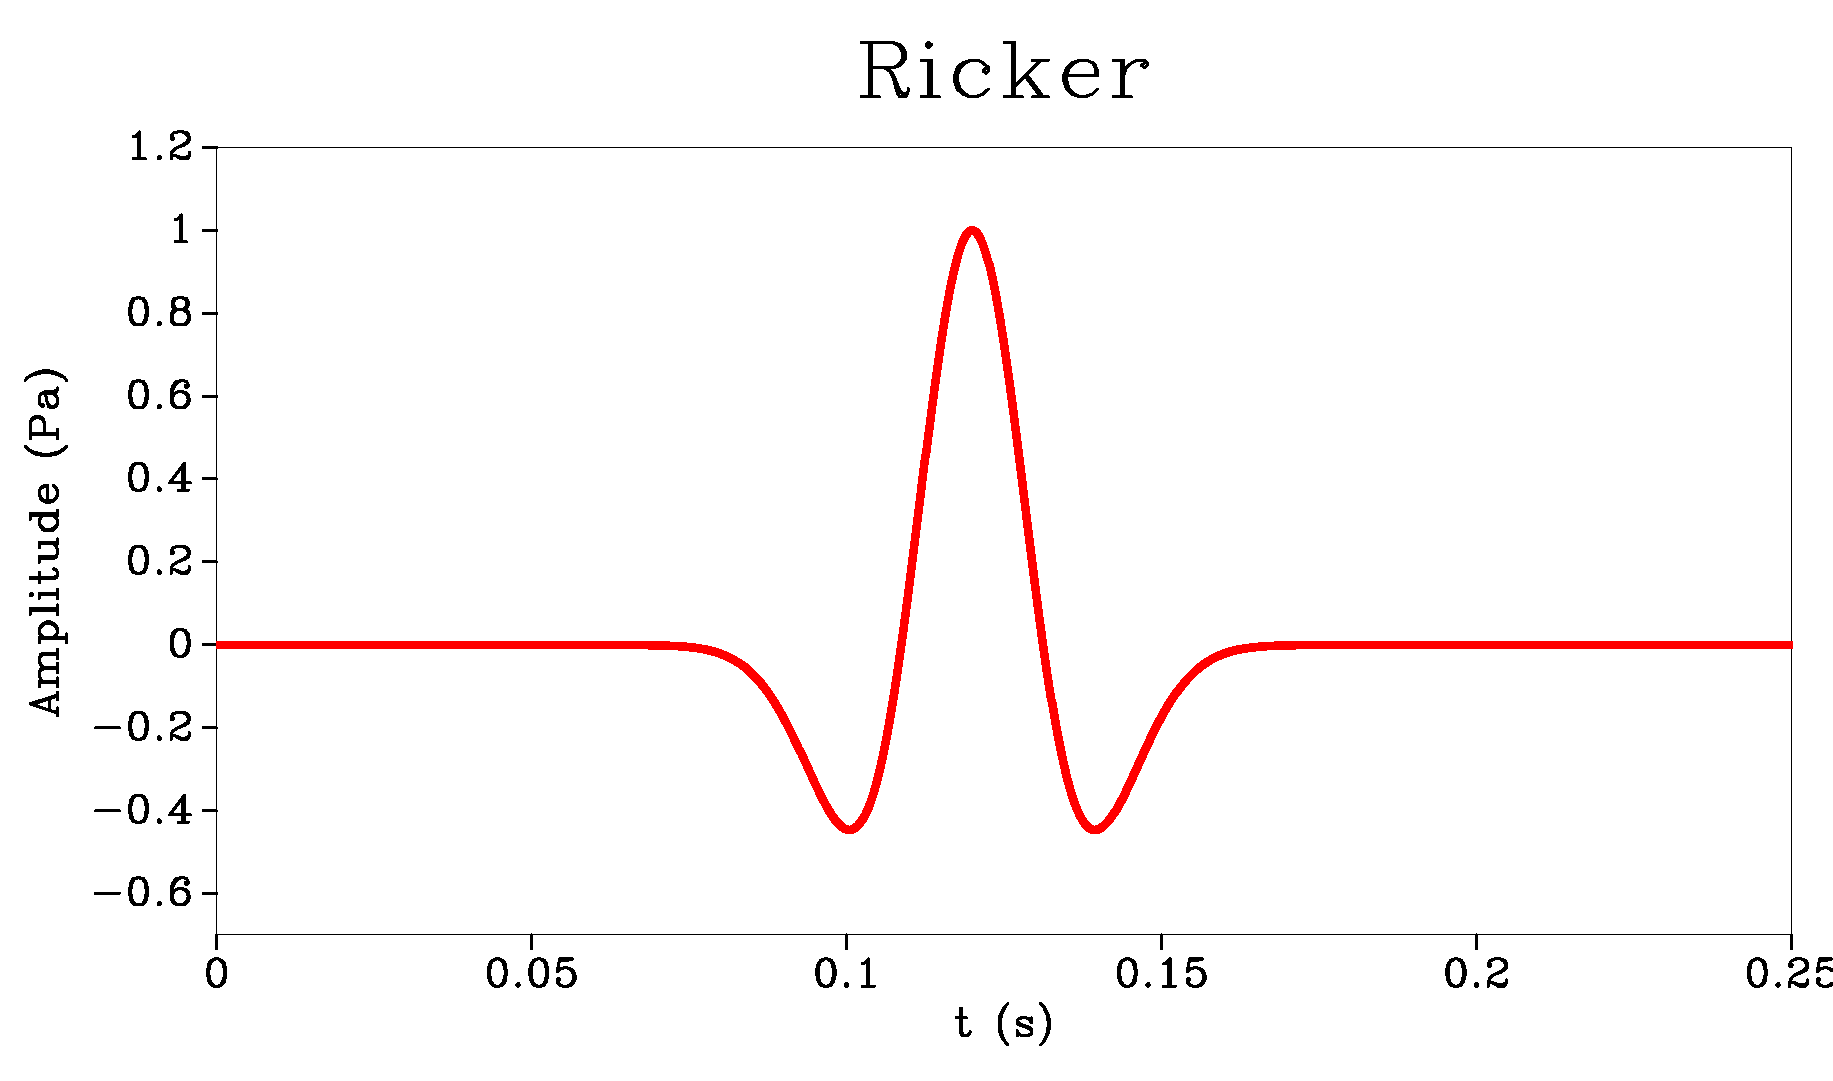
\includegraphics[width=15cm]{wav1}
	\caption{Assinatura da fonte usada: Ricker com frequência pico de $12~Hz$.} 
	\label{fig:ricker}
\end{figure} 

\section{M\'etodo das diferenças finitas}


Para encontrar a evolução do campo de onda, deve-se discretizar as equa\c{c}\~oes 
(\ref{eq.onda}). Esta será feita utilizando-se o método das diferenças 
finitas, que é caracterizado por substituir as derivadas de uma equação 
diferencial por expressões algébricas de diferenças. Essas expressões podem ser 
obtidas a partir do truncamento da expansão em série de Taylor e a ordem do erro 
da aproximação da derivada é função desse truncamento. 

A aplicação do método das diferenças finitas é realizada considerando o 
domínio discretizado em um \textit{grid} retangular de pontos, geralmente 
equiespaçados. Essa característica dificulta sua aplicação em domínios curvos. 
No entanto, este método possui uma boa acurácia e é de fácil implementação 
\citep{snieder1998}. Um problema é 
que o método não permite que se tenham \textit{grids} com refinamentos 
diferentes sobre o domínio \citep{zakaria2000two}. 


Esse método de discretização pode ser aplicado na 
equação da onda acústico vetorial.  Portanto, sabendo que é 
uma equação de primeira ordem, pode-se fazer a seguinte aproximaç\~ao centrada  para a 
derivada em rela\c{c}\~ao \`a $t$


\begin{equation}
\DDt[f(t)] \approx \frac{f(t+\Delta t)-f(t-\Delta t)}{2\Delta t} \label{eq:dif}
\end{equation} 
onde $f(t)$ é uma função qualquer e $\Delta t$ a diferença entre pontos consecutivos no tempo.
Para as outras diferenças finitas, progressiva e regressiva, tem-se as seguintes relações, respectivamente:
\begin{equation}
\DDt[f(t)] \approx \frac{f(t+\Delta t)-f(t)}{\Delta t} \label{eq:difp},
\end{equation}
\begin{equation}
\DDt[f(t)] \approx \frac{f(t)-f(t-\Delta t)}{\Delta t} \label{eq:difr},
\end{equation}

Para as equações (\ref{eq:dif}), (\ref{eq:difp}) e \ref{eq:difr}, foi utilizada a expansão da derivada de primeira ordem. Com o intuito de fazer a discretização em relação ao espaço, será substituído os termos $t$ e $\Delta t$ destas equações por $x$
e $\Delta x$. Sendo $x$ a variável espacial e o $\Delta x$ a diferença entre pontos consecutivos no espaço. 
\subsection{Cálculo dos coeficientes}
Para encontrar os coeficientes das diferenças finitas, foi utilizada a seguinte equação:
\begin{equation}
K\delta_{K,1}=2\sum_{j=0}^{N-1}d_j\Big(\frac{2j+1}{2}\Big)^K, \quad K=1, 3,...,2N \label{eq:coef}
\end{equation}
sendo que a solução deste sistema linear determina os coeficientes $d_j$ para uma aproximação de ordem 2N.
\section{Discretização da equação da onda}


Para encontrar a evolução do campo de onda, deve-se discretizar a equação 
(\ref{eq.onda}). Esta será feita utilizando-se o método das diferenças 
finitas. Portanto, sabendo que é 
uma equação de segunda ordem, pode-se fazer a seguinte aproximaç\~ao para a 
derivada parcial em rela\c{c}\~ao \`a $x$:
\begin{equation}
\frac{\partial^2P(x,z,t)}{\partial x^2}\approx\frac{P_{i+1,j}^{l}-2P_{i,j}^{l}+P_{i-1,j}^{l}}{\Delta x^2}, \label{dx2}
\end{equation}
onde $P_{i,j}^{l} = P(x_i,z_j,t_l)$ e $x_i = x_0 + i\Delta x$, $z_j = z_0 + 
j\Delta z$, e $t_l = t_0 + l\Delta t$. Esta \'e uma aproximação de segunda ordem. Pode-se, de maneira an\'aloga aproximar as segundas derivadas em $z$ e $t$.

Substituindo em (\ref{eq.onda}) as derivadas por suas aproxima\c{c}\~oes de diferen\c{c}as finitas e isolando o termo $P_{i,j}^{l+1}$, temos 
\begin{equation}
\begin{aligned}
P_{i,j}^{l+1}=c^2\frac{\Delta t^2}{\Delta h^2}(P_{i+1,j}^{l}+P_{i-1,j}^{l}+P_{i,j+1}^{l}+P_{i,j-1}^{l}-4P_{i,j}^{l}) \\
+ 2P_{i,j}^{l}-P_{i,j}^{l-1} - c^2 \Delta t S_{i,j}^l, \label{desenvol2}
\end{aligned}
\end{equation}

\section{Relação de dispersão}

Assumindo a propaga\c{c}\~ao de uma onda plana em um meio homog\^eneo, temos:
\begin{equation}
P_{i,j}^{l}=e^{i(k_{x}x_{i}+k_{z}z_{j}-\omega t_{l})}. \label{pij}
\end{equation}
A partir desta equação é possível determinar as seguintes relações:
\begin{eqnarray}
P_{i\pm1,j}^{l}&=&e^{i[k_{x}(x_{i}\pm\Delta x)+k_{z}z_{j}-\omega t_{l}]} \nonumber \\
&=&e^{\pm ik_{x}\Delta x}e^{i(k_{x}x_{i}+k_{z}z_{j}-\omega t_{l})} = e^{\pm ik_{x}\Delta x}P_{i,j}^{l}. \label{eq:Pi1}
\end{eqnarray}
De modo an\'alogo
\begin{equation}
P_{i,j\pm1}^{l}=e^{\pm ik_{z}\Delta x}P_{i,j}^{l}, \label{eq:Pj1}
\end{equation}
e 
\begin{equation}
P_{i,j}^{l\pm1}=e^{\mp i\omega\Delta t}P_{i,j}^{l}.\label{eq:Pt1}
\end{equation}
% \begin{equation}
% P_{i\pm1,j}^{l}=e^{\pm ik_{x}\Delta x}e^{i(k_{x}x_{i}+k_{z}z_{j}-\omega t_{l})} 
% \label{imp}
% \end{equation}
Substituindo as equações (\ref{eq:Pi1}), (\ref{eq:Pj1}) e (\ref{eq:Pt1}) em 
(\ref{desenvol2}), considerando $S_{i,j}^l=0$, tem-se que:
\begin{eqnarray}
e^{-i\omega\Delta t}P_{i,j}^{l}+e^{i\omega\Delta t}P_{i,j}^{l} 
&=&c^2\frac{\Delta t^2}{\Delta x^2}(e^{+ ik_{x}\Delta h
}P_{i,j}^{l}\\ \nonumber
& &+e^{- ik_{x}\Delta h}P_{i,j}^{l}+e^{+ik_{z}\Delta h}P_{i,j}^{l}\\ \nonumber
& &+e^{-ik_{z}\Delta h}P_{i,j}^{l}-4P_{i,j}^{l})+2P_{i,j}^{l}. 
\end{eqnarray}
A partir da relação de Euler para cosseno,
\begin{equation}
\cos(y)=\frac{e^{iy}+e^{-iy}}{2} \label{euller},
\end{equation}
podemos chegar na seguinte equação
% \begin{equation}
% 2\cos(y)=e^{iy}+e^{-iy} \label{euller2}.
% \end{equation}
% Substituindo a relação (\ref{euller2}) em (\ref{desen3}), podemos chegar na 
% seguinte equação:
% %Erro na numeração, n puxou o do eqnarray
\begin{equation}
\cos(\omega \Delta t) =c^2\frac{\Delta t^2}{\Delta h^2}(\cos(k_{x}\Delta h) + \cos(k_z\Delta h)-2) + 1.
\label{eq:disp1}
\end{equation}
Sendo $k = \frac{\omega}{c}$ o n\'umero de onda, podemos definir $k_x = k\sin \theta$ e $k_z = k \cos \theta$, onde $-\pi < \theta < \pi$ \'e a dire\c{c}\~ao de propaga\c{c}\~ao da onda plana em rela\c{c}\~ao ao eixo vertical, orientado para baixo. Com isso, Equação (\ref{eq:disp1}) fica
\begin{equation}
\cos(\omega \Delta t)=c^2\frac{\Delta t^2}{\Delta h^2}(\cos(k\sin \theta\Delta h) + \cos(k \cos\theta\Delta h)-2)+ 1.
\label{eq:disp2}
\end{equation}

Da eq. (\ref{eq:disp2}) podemos escrever 
\begin{eqnarray}
\omega (k,\theta)&=&\frac{1}{\Delta t} \cos^{-1}\Big\{ c^2\frac{\Delta t^2}{\Delta h^2}(\cos(k\sin \theta\Delta h) \nonumber\\ 
&&+ \cos(k \cos\theta\Delta h)-2)+ 1\Big\}.
\label{eq:disp3}
\end{eqnarray}
Desta equa\c{c}\~ao podemos escrever as express\~oes para velocidade de fase ($c_p$) e de grupo ($c_g$):
\begin{eqnarray}
c_p (f,\theta)\hspace{-8pt}&=&\hspace{-8pt}\frac{c}{2\pi f\Delta t} \cos^{-1}\Bigg\{ c^2\frac{\Delta t^2}{\Delta h^2}\left(\cos\left(\frac{2\pi f}{c}\sin \theta\Delta h\right)\right. \nonumber\\ 
&&+ \left.\cos\left(\frac{2\pi f}{c} \cos\theta\Delta h\right)-2\right)+ 1\Bigg\}
\label{eq:cp}
\end{eqnarray}
e
\begin{eqnarray}
c_g(f,\theta) &=& \Bigg(\frac{c^2\Delta t}{\Delta h} \left[ \sin(k\sin \theta\Delta h) \sin \theta \right. \nonumber \\ 
&& \left. + \sin(k\cos \theta\Delta h)\cos \theta\right]\Bigg) \times \nonumber \\
&& \Bigg(1 - \Big\{ c^2\frac{\Delta t^2}{\Delta h^2}(\cos(k\sin \theta\Delta h) \nonumber\\ 
&&+ \cos(k \cos\theta\Delta h)-2)+ 1\Big\}^2\Bigg)^{-1/2}.
\label{eq:cg}
\end{eqnarray}

A partir dessas equações, é possível gerar e ajustar gráficos com a velocidade de fase e de grupo, apresentados na Figura \ref{fig:disp}. 

\begin{figure}[ht!]
	\centering
	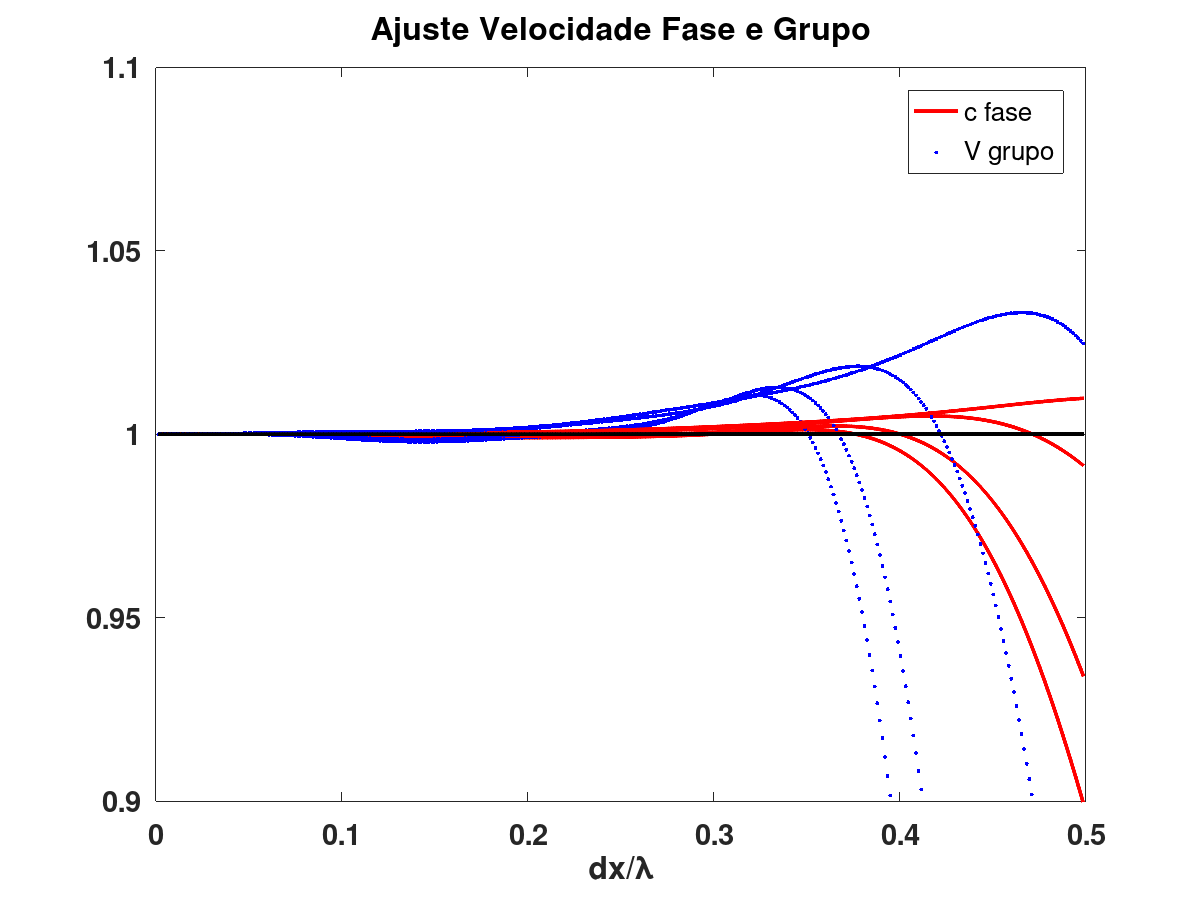
\includegraphics[width=11cm]{disper}
	\caption{Relação de dispersão, considerando ajustes na velocidade de fase e de grupo. Cada par de curvas está associado a um ângulo de propagação da onda plana.}
	\label{fig:disp}
\end{figure}

\section{Bordas de absorção}
Em uma solu\c{c}\~ao num\'erica, o meio de propaga\c{c}\~ao \'e finito. Assim, 
condi\c{c}\~oes de contorno devem ser aplicadas nas bordas do modelo. Estas causam, invariavelmente, reflex\~ao. 
Os dados que são refletidos pela borda ocasionam erros para os dados sísmicos
modelados, misturando o dado da propagação no meio com as reflex\~oes nas 
fronteiras do modelo. Com o intuito de retirar este efeito, deve ser aplicada 
uma borda absorvente, cujo objetivo é diminuir ou tirar a influência da 
reflexão das bordas \citep{komatitsch2007unsplit}.


\subsection{PML(Perfect Matched Layer)}

Com a finalidade de simular um meio ilimitado, \cite{berenger1994perfectly} introduziu a PML
(perfect Matched Layer), uma borda adicional em torno do meio limitado (Fig. \ref{fig:borda}) com amortecimento do campo de onda que chega nos limites
do modelo a fim de evitar as reflexões dos mesmos e, assim, interferir no sinal registrado. Na Figura \ref{fig:borda}, o $\sigma$ se refere ao amortecimento do campo de onda
que age apenas na região da borda.

\begin{figure}[ht!]
	\centering
	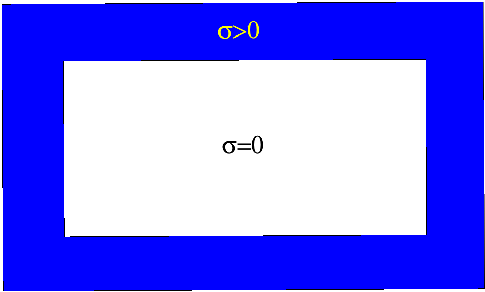
\includegraphics[width=11cm]{borda}
	\caption{Bordas adicionadas em volta de um modelo limitado para simular um meio
		ilimitado no processo de modelagem.}
	\label{fig:borda}
\end{figure}

Na Figura \ref{fig:borda}, o termo $\sigma$ pode ser definido da seguinte forma
\begin{equation}
\sigma(x)=\left\{\begin{matrix} 0 & \text{no dominío de interesse}  \\
\frac{3}{2}\text{log}(\frac{1}{R})c_{max}\Delta(\frac{x}{L}) & \text{nas bordas}, \\
\end{matrix}\right. \label{eq:sigma}
\end{equation}
sendo $R$ o coeficiente de reflexão desejado para incidência normal, $L$ a largura da banda de absorção e $f_{pico}$ a frequência pico do pulso.

Além de utilizar essa Equação \ref{eq:sigma},   tem-se uma implementação simples utilizando a seguinte equação:

\begin{equation}
\dddtt[p]+\sigma(x,y)\ddt[p]=c^2\nabla^2p, \label{eq:simples}
\end{equation}
sendo 
\begin{equation}
\sigma(x,y)=\lambda(x)+\lambda(y),
\end{equation}
com 
\begin{equation}
\lambda(x)=\left\{\begin{matrix} 0 & \text{no dominío de interesse}  \\
\pi f_{pico}\Delta (\frac{x}{L}) ^2& \text{nas bordas}, \\
\end{matrix}\right. \label{eq:lambda}
\end{equation}

A partir da Equação \ref{eq:simples}, pode-se reescrever \ref{desenvol2} da seguinte forma:
\begin{equation}
\begin{aligned}
p(x,z,t+\Delta)-2p(x,z,t)+p(x,z,t-\Delta)+\Delta\frac{\lambda(x)+\lambda(z)}{2}\{p(x,y,t+\Delta) \\
-p(x,y,t-\Delta)\}\\
=\Big{(}\frac{c(x,z)\Delta}{h}\Big{)}^2\{2d_0p(x,z,t) \\
+ \sum_{j=1}^{N-1}d_j(p(x+jh,z,t)+p(x-jh,z,t))\\
+ \sum_{j=1}^{N-1}d_j(p(x,z+jh,t)+p(x,z-jh,t))\} \\
+\Delta t^2S(t)\delta_{BL}(\vc{x}-\vc{x_s})+O(\Delta t^2,h^{2N})
\end{aligned}
\end{equation}

\section{RTM}
 
A técnica da Migração Reversa no Tempo consiste em propagar o sinal do tempo final para o tempo inicial, na qual é aplicada uma
condição de imagem para obter a imagem em profundidade. Essa técnica de imageamento vantagens quando comparado com outras
técnicas por solucionar a equação de onda completa da onda e viabilizar o imageamento de
estruturas mais complexas \citep{matias}.

\begin{equation}
	I(\vc{x})=\sum_{s}\int_{0}^{T}\sum_{r}p_s(\vc{x},t;\vc{x}_S)p_r(\vc{x},t;\vc{x}_r)dt,
\end{equation}
na qual $I(\vc{x})$ é a imagem final migrada para cada ponto, $\vc{x}_S$ é a posição da fonte, $\vc{x}_r$ é a posição do receptor, $T$ é o tempo total de registro, $p_s$ o campo de onda que inicia na fonte e $p_r$ o retropropagado pelos receptores.

\section{Paralelização}

É necessário frequentemente utilizar diversas unidades de processamento para obter o poder computacional desejado para resolver alguns problemas. A fim de atender a essa demanda, foram criados sistemas que possuem essas diversas unidades de processamento, objetivando aumentar a capacidade de computação ao menor custo possível. A um sistema com diversas dessas unidades se dá o nome de \textit{cluster}. Cada um dos processadores de um \textit{cluster} é chamado de nó.

Paralelizar um processamento de dados é dividir o esforço computacional entre diversos processadores e fazer com que isso ocorra de forma aproximadamente simultânea \citep{chandra2001parallel}. A paralelização pode ser implementada através de uma divisão do bloco inicial de dados em blocos menores que podem ser processados individualmente, simultaneamente e em menos tempo do que o bloco inicial. Ao final, os dados oriundos dos diversos processamentos devem ser agregados para se obter o resultado final. Uma paralelização pode ser implementada e executada num sistema paralelo ou em um sistema distribuído. 

As complicações referentes a paralelização podem ocorrer devido a divisão de trabalho entre os processadores, garantir que os passos sequenciais estejam sendo executados de forma correta e garantir exclusão mútua no acesso aos recursos. Para resolver esses problemas, a forma é garantir a sincronização dos processos envolvidos. 

